% !TeX root = ./main.tex
\documentclass[main]{subfiles}
\begin{document}
\chapter{Непрерывные отображения}
\section{Непрерывные отображения}
\begin{definition}
    $(X, \rho), (Y, d)$ -- метрические пространства. $f: X \to Y$ -- отображение.
    Говорим, что $f$ непрерывно в $x_0 \in X$, если
    $\forall \epsilon > 0\ \exists \delta > 0:$ если $\rho(x_1, x_0) < \delta \implies d(f(x_0), f(x_1)) < \epsilon$.
\end{definition}
\begin{definition}
    $f$ непрерывно если $f$ непрерывно в любой точке.
\end{definition}
\begin{remark}
    $f: X \to Y$ непрерывно в $x_0 \Leftrightarrow \forall \epsilon > 0\ \exists \delta > 0:$
    $f\left(B_X(x_0, \delta)\right) \subset B_Y(f(x_0), \epsilon)$.
\end{remark}

\begin{definition}
    $(X, \Omega_X)$ и $(Y, \Omega_Y)$ -- топологические пространства.
    $f: X \to Y$ -- отображение.
    $f$ называется непрерывным в точке $x_0 \in X$, если $\forall U \in \Omega_Y : f(x_0) \in U\ \exists V \in \Omega_X: x_0 \in V: f(V) \subset U $
\end{definition}

\begin{theorem}
    $(X, \rho)$ и $(Y, d)$ метрические пространства. $f: X \to Y$ отображение.
    $f$ непрерывно $\Leftrightarrow \forall U \subset Y$, $U$ открыто, $f^{-1}(U)$ открыто в $X$.
\end{theorem}
\begin{proof}
    Прямое доказательство: $f$ непрерывное, т.е.
    $\forall x_0\ \forall \epsilon > 0\ \exists \delta(\epsilon, x_0) > 0: f(B_X(x_0, \delta))\subset B_Y (f(x_0), \epsilon)$.
    $\forall U \subset Y$ -- открыто, $V \coloneqq f^{-1}(U)$.
    Хотим доказать, что $V$ открыто. $\forall x_0 \in V \implies f(x_0) \in U$.
    $U$ -- отрытое, значит $\exists \epsilon > 0: B(f(x_0), \epsilon) \subset U$.
    Тогда $\exists \delta > 0: f(B_X(x_0, \delta)) \subset B_Y(f(x_0), \epsilon) \subset U$.
    Если $f(B_X(x_0, \delta)) \subset U \implies B_X(x_0, \delta) \subset V$.

    Обратное: $\forall x_0 \in X, \forall\epsilon >0.$ $U\coloneqq B(f(x_0); \epsilon)$ открытое.
    Значит $f^{-1}(U)$ открыт, $x_0 \in f^{-1}(U)$, т.к. $f(x_0) \in U$.
    Тогда $\exists \delta > 0: B(x_0, \delta) \subset f^{-1}(U)$.
    $f(B(x_0), \delta) \subset U \coloneqq B(f(x_0), \epsilon)$.
\end{proof}

\begin{definition}
    $(X, \Omega_X)$ и $(Y, \Omega_Y)$ -- топологические пространства.
    $f: X \to Y$ -- отображение.
    $f$ называется непрерывным, если $\forall U \in \Omega_Y\ f^{-1}(U) \in \Omega_X$.
\end{definition}

\begin{remark}
    $X, Y$ -- множества, $A, B \subset X; C, D \subset Y$.
    \begin{gather*}
        f(A \cup B) = f(A) \cup f(B)\\
        f(A \cap B) = f(A) \cap f(B)\text{ -- неверно!}\\
        f^{-1} (C \cup D) = f^{-1}(C) \cup f^{-1}(D)\\
        f^{-1} (C \cap D) = f^{-1}(C) \cap f^{-1}(D)
    \end{gather*}
    Почему неверно второе:
    \begin{gather*}
        f(A \cap B) = \{f(x_0) : x_0 \in A \cap B\} \\
        \begin{multlined}
            f(A) \cap f(B) = \{f(x_0) : x_0 \in A\} \cap \{f(y_0) : y_0 \in B\} =\\
            \{f(x_0) = f(y_0) : x_0 \in A, y_0 \in B\}
        \end{multlined}
    \end{gather*}
    Почему неверны остальные -- упражнение.
\end{remark}

\begin{definition}
    $f: X \to Y$ называется
    \begin{enumerate}
        \item непрерывным,  если прообраз открытого множества открыт
        \item непрерывным, если прообраз замкнутого замкнут
        \item открытым, если образ открытого открыт
        \item замкнутым, если образ замкнутого замкнут
    \end{enumerate}
\end{definition}

$F \subset X$ замкнутое, $U \coloneqq Y \setminus F$ открытое.
$f^{-1} (Y\setminus U) = X \setminus f^{-1}(U)$ замкнуто, если $U$ открыто.
$f^{-1} (U)$ и $f^{-1}(Y \setminus U )$ не пересекаются и в объединении дают $X$.

\begin{example}
    $X=Y=\R$, на $X$ дискретная топология, на $Y$ стандартная, $f: X \to Y$, $f(x) = x$ непрерывно,
    но не открытое и не замкнутое.

    $U$ подмножество, не открытое в стандартной топологии, но открытое в дискретной.
\end{example}

\begin{example}
    Разница между открытым и замкнутым:
    рассмотрим отображения включения: $i: U \hookrightarrow X, i(x) = x$.
    Если
    \begin{itemize}
        \item $U$ открытое множество, тогда $i$ открытое
        \item $U$ не открытое в $X$, тогда $i$ не открытое отображение
        \item $U$ замкнутое множество в $X$, тогда $i$ замкнутое
    \end{itemize}
\end{example}

\section{Гомеоморфизмы}

\begin{definition}
    $f: X \to Y$ называется гомеоморфизмом, если
    \begin{enumerate}
        \item $f$ непрерывно
        \item $f$ биективно
        \item $f^{-1}$ непрерывно
    \end{enumerate}
\end{definition}

\begin{example}
    $X=Y=\R$, на $X$ дискретная топология, на $Y$ стандартная.

    $f: X \to Y; f(x)=x$, $f$ непрерывно и биективно, но не $f^{-1}$ не непрерывно, не гомеоморфизм!
\end{example}
\begin{example}
    $X = [0, 2\pi)$, $Y = S' = \{z\in \C: |z| = 1\}$

    $f: X \to Y; f(t) = e^{it}$ -- биекция и непрерывное отображение, но обратное не непрерывно:
    \begin{center}
        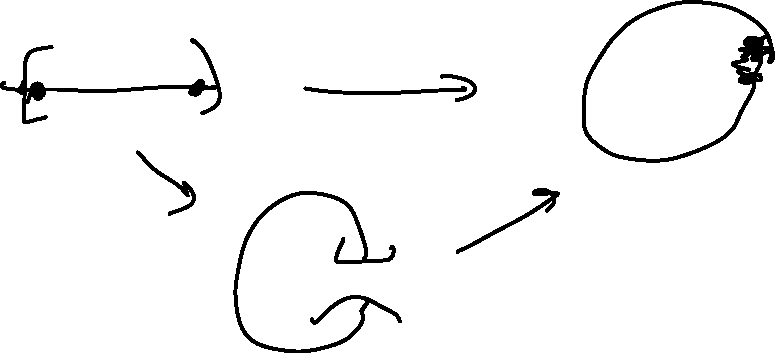
\includegraphics[width=0.7\linewidth]{not_homeomorphism.pdf}
    \end{center}
\end{example}

\begin{theorem}
    \begin{enumerate}
        \item Гомеоморфность, т.е. существование какого-то гомеоморфизма, есть эквивалентность
        \item $f:X \to Y$ -- гомеоморфизм, тогда $f$ индуцирует биекцию между $\Omega_X$ и $\Omega_Y$ (и между замкнутыми множествами $X$ и $Y$ тоже)
    \end{enumerate}
\end{theorem}

\begin{proof}
    Докажем 1: будем означать гомеоморфность символом эквивалентности: $\sim$.
    Пусть $X \sim X, id: x \mapsto x$. $id(X) = X$.
    Пусть $X \sim Y \implies \exists f: X \to Y$ -- гомеоморфизм, тогда $f^{-1}: Y \to X$ -- гомеоморфизм.
    Пусть $X \sim Y, Y \sim Z \implies X \sim Z$. $f: X \to Y, g: Y \to Z, g \circ f: X \to Z$ -- гомеоморфизм.

    Доказательство 2 очевидно
\end{proof}

\begin{example}
    $(0,1) \overset{f}{\sim} (a,b) \overset{g}{\sim} \R \overset{\text{упр}}{\sim} (0, +\infty)$
    \begin{gather*}
        g: \left(- \frac{\pi}{2};\frac{\pi}{2}\right) \to \R; g(x) = \tg x\\
        f(0,1) \to (a,b); f(x) = (b-a)x + a
    \end{gather*}

    Но $(0,1) \not\sim [0,1]$. Почему? Нужно искать инварианты.
\end{example}

\begin{example}
    Шуточные примеры:
    \begin{center}
        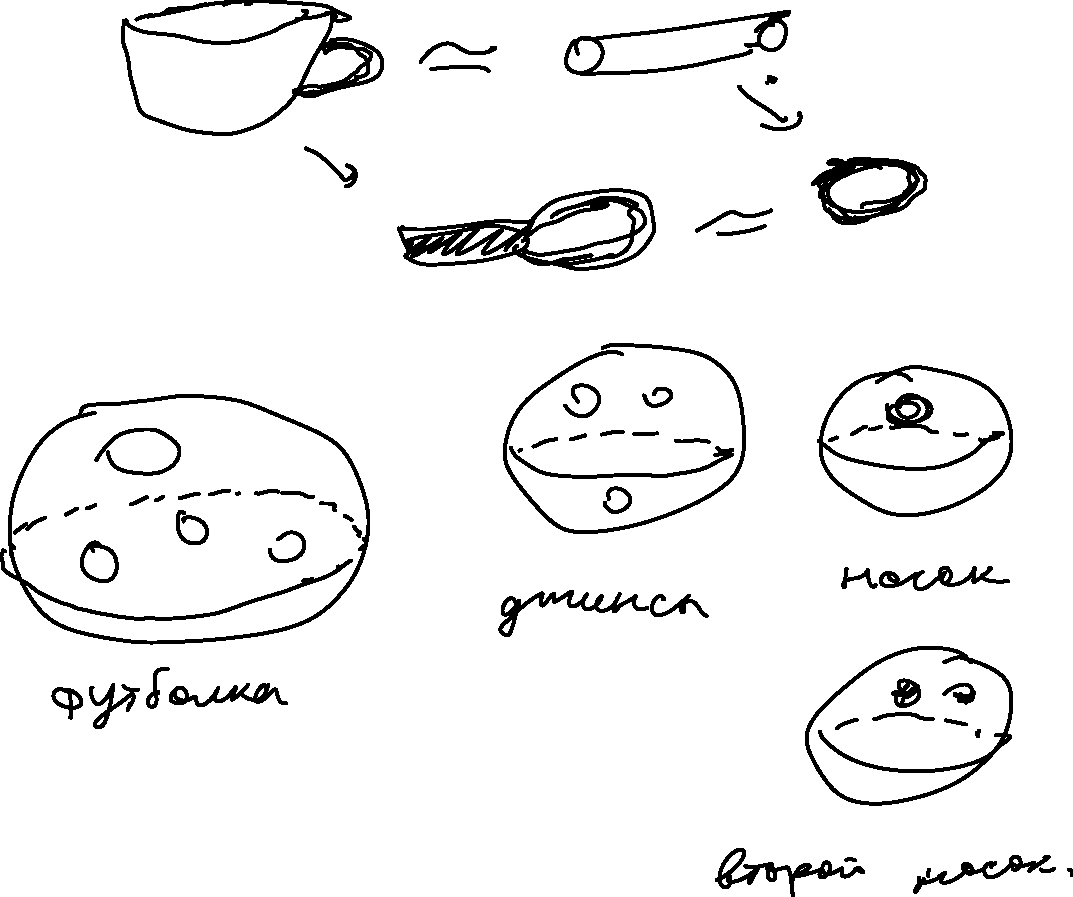
\includegraphics[width=0.7\linewidth]{joke_homeomorphism.pdf}
    \end{center}
\end{example}

\section{Инициальная топология}
\subsection{Прообраз топологии}

$f: X \to Y$ отображение, $(Y, \Omega_Y)$ топологическое пространство. $X$ пока нет.
Цель: ввести топологию на $X$, т.ч. $f$ непрерывно, топология на $X$ слабейшая из возможных.

\begin{definition}
    $(X, \Omega_1)$ и $(X, \Omega_2)$ топологические пространства.
    Говорим, что $\Omega_1$ сильнее $\Omega_2$, если $\Omega_2 \subset \Omega_1$.
\end{definition}

\begin{definition}
    Самая слабая топология на $X$, т.ч. $f:X\to Y$ непрерывно, называется прообразом топологии $\Omega_Y$
\end{definition}

\begin{theorem}
    Прообраз топологии существует.
\end{theorem}
\begin{proof}
    $U \in \Omega_Y \implies f^{-1}(U)$ должен быть открыт в $X$.
    Прообраз $\Omega_X \coloneqq \{f^{-1}(U) : U \in \Omega_Y\}$.
    \begin{gather*}
        f^{-1}(U_1 \cap U_2) = f^{-1}(U_1) \cap f^{-1}(U_2)\\
        f^{-1}\left(\bigcup_{i \in I} U_i\right) = \bigcup_{i \in I} f^{-1}(U_i)\\
        f^{-1}(\varnothing) = \varnothing, f^{-1}(Y) = X.
    \end{gather*}
\end{proof}

Важный частный случай: $(X, \Omega_X)$ -- топологическое пространство. $Y \subset X$.
$i: Y \hookrightarrow X$. Тогда $Y$ наделяется топологией.

\begin{definition}
    Такая топология на $Y$ называется индуцированной.
\end{definition}
$V \subset Y$. $V$ открыто в $Y$ если $\exists U$ -- открытое в $X$: $i^{-1}(U) = V = U \cap Y$.

\begin{definition}
    Переформулируем: $V \subset Y$ называется открытым, если $\exists U$ -- открытое в $X: U \cap Y = V$.
\end{definition}

\begin{remark}
    $V$ открыто в $Y$, но это не означает, что $V$ открыто в $X$.

    $Y = [0,1], X = \R$ cо стандартной топологией.
    $U = (-1, 0.5)$ открыто в $\R = X$.
    $U \cap [0,1] = [0, 0.5)$ открыто в $Y$, но не открыто в $X$.
\end{remark}

\subsection{Инициальная топология}
\begin{definition}
    $X$ -- множество. $(Y_i, \Omega_i)$ -- топологические пространства.
    $f_i: X \to Y_i$.
    Хотим завести на $X$ топологию, такую что все $f_i$ непрерывные, а топология на $X$ слабейшая из возможных.
    Такая топология называется инициальной.
\end{definition}

\begin{theorem}
    Инициальная топология существует и единственна.
\end{theorem}
\begin{proof}
    $f^{-1}_i(U_i)$ должны быть открытыми, $U_i \subset Y_i$ открытые.
    Все такие множества -- предбаза.
    По критерию базы:
    \[\mathfrak{B} = \{f^{-1}_{i_1} (U_{i_1}) \cap ... \cap f^{-1}_{i_k} (U_{i_k}) : U_{i_j} \in \Omega_j\}\]
    является базой некоторой топологии.
\end{proof}

\begin{example}
    $(X, \Omega_X)$ и $(Y, \Omega_Y)$ -- топологические пространства.
    Как ввести топологию на $X \times Y$?
    Берем проекции на $X$ и $Y$ и инициальную топологию.
    Как ее описать? Далее.
\end{example}

\subsection {Бесконечное произведение. Ликбез}

$\{X_i\}_{i \in I}$ -- семейство множеств.
Пусть $(X_i, \Omega_i)$ -- топологические пространства.
\[\prod_{i \in I} X_i\ = \{f: I \to \bigcup_{i \in I} X_i: f(j) \in X_j\}\]

Пусть $\forall i\ X_i \neq \varnothing$. Почему $\prod_{i \in I} X_i \neq \varnothing$?
Это равносильно аксиоме выбора.

\begin{axiom}[выбора]
    $\{X_i\}_{i \in I}$ -- семейство непустых множеств.
    Тогда $\exists Y$ состоящее из элементов $X_i$ (по одному элементу из каждого множества)
\end{axiom}
\begin{lemma}[Цорна]
    $X$ -- непустое частично упорядоченное множество (введено отношение порядка, которое рефлексивно, антисимметрично и транзитивно).
    $\forall x_1 \le x_2 \le ...\ \exists x_*: x_* > x_i \forall i$, тогда
    в множестве $X$ существует максимальный элемент
\end{lemma}
\begin{theorem}[Цермело]
    Любое непустое множество можно вполне упорядочить (ввести такой порядок, что любое подмножество будет иметь наименьший элемент).
\end{theorem}

Стандартное $\le$ на $\R$ -- неполный порядок, например $(0, 1)$ не имеет наименьшего.

\begin{assertion}
    Аксиома выбора $\Leftrightarrow$ лемме Цорна $\Leftrightarrow$ теореме Цермело.
\end{assertion}

\begin{theorem}
    У любого векторного пространства есть базис.
\end{theorem}
\begin{proof}
    $A$ -- множество всех ЛНЗ наборов. $(A; \subset )$ -- частично упорядоченное множество.
    \[x_1 \subset x_2 \subset ... \implies x_* = \bigcup_{i=1}^\infty X_i\]
    по лемме Цорна существует максимальный элемент. Он и является базисом.
\end{proof}


\subsection{Декартово произведение}

\begin{center}
    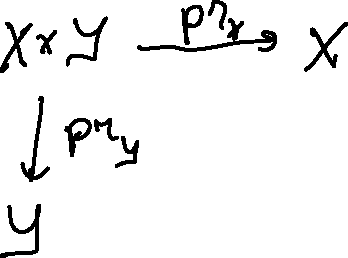
\includegraphics[width=0.5\linewidth]{projection.pdf}
\end{center}
Есть $X \times Y$, $p_X(x,y) = x$, $p_Y(x,y)=y$

$(X, \Omega_X), (Y, \Omega_Y)$ -- топологические пространства.
На $X\times Y$ введем топологию (инициальную).
$U \subset X$ открыто $p_X^{-1}(U) = U \times Y$.
$V \subset Y$ открыто $p_Y^{-1}(V) = X \times V$.
\begin{gather*}
    (U_1 \times Y) \cap (U_2 \times Y) = (U_1 \cap U_2) \times Y\\
    (U \times Y) \cap (X\times V)  = U \times V
\end{gather*}
Таким образом $\{U \times V : U \in \Omega_X; V \in \Omega_Y\}$ -- база топологии $X\times Y$

Иначе: множество $W \subset X\times Y$ является открытым, тогда и только тогда, когда
$\forall (x_0, y_0) \in W\ \exists U_{x_0} \in \Omega_X, V_{y_0} \in \Omega_Y: x_0 \in U_{x_0},
    y_0 \in V_{y_0}, U_{x_0} \times V_{y_0} \subset W$

\begin{example}
    Это совпадает с топологией на $\R^2$:
    \begin{center}
        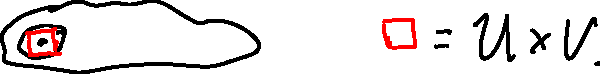
\includegraphics[width=0.7\linewidth]{open_R2.pdf}
    \end{center}
\end{example}
\begin{example}
    \

    \begin{center}
        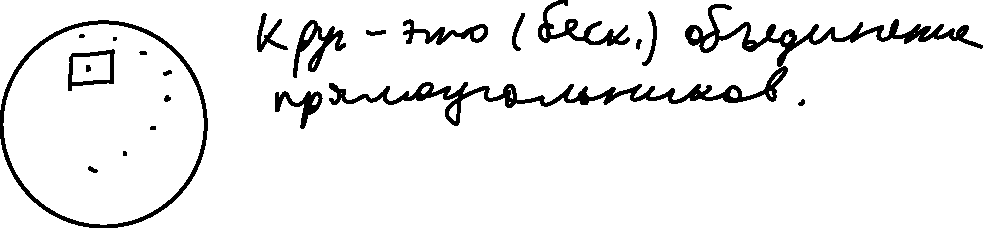
\includegraphics[width=0.7\linewidth]{open_circle.pdf}
    \end{center}
\end{example}


$\prod_{i \in I} X_i$ хотим снабдить топологией.
$U \subset X_i$ -- открыто, тогда $U \times \prod_{j \neq i} X_j$ -- открытое
множество в инициальной топологии. Такие множества предбаза.
\[U_1 \times U_2 \times ... \times U_k \times \prod_{j \neq 1, ..., k} X_j\]
--  база топологии.

НО $U_i \subset X_i$ открыто, $\prod U_i$ не является открытым в $\prod X_i$!

\begin{property}
    Если на $X_i$ дискретная топология, то $\prod_{i \in I} X_i$ не является
    дискретным пространством, если $I$ бесконечно
\end{property}
В частности счетное произведение $\{0,1\} \times \{0,1\} \times ... = \{0, 1\}^{\N}$ не дискретно.
Такое множество гомеоморфно $K$ -- канторову множеству.
\begin{center}
    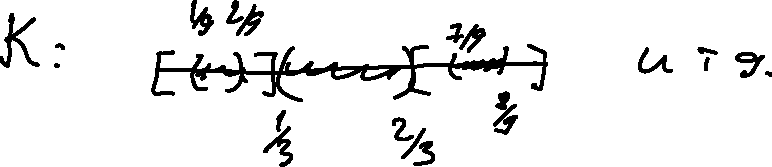
\includegraphics[width=0.7\linewidth]{K.pdf}
\end{center}
\begin{property}
    \begin{enumerate}
        \item $l(K) = 0$. $l(K) = 1 - (1/3 + 2/9 + 4/27 + ...)$
        \item $K$ замкнуто
        \item $K$ состоит из чисел без 1 в троичной записи. $1/3 = 0.1 = 0.022222...$ в троичной записи
        \item $K \simeq \{ 0,1 \}^{\N}$ -- гомеоморфизм.
              $K = \{0.a_1a_2a_3...: a_i \in \{0,2\}\}$ (не очень простое упражнение)
        \item  $K$ несчетно
        \item $K \simeq K \times K$,
              по пункту 4: $\{0,1\}^{\N} \times \{0,1\}^{\N} = \{0,1\}^{\N^2}$, а $\N^2 \sim \N$,
              поэтому $\{0,1\}^{\N^2} \simeq \{0,1\}^{\N}$
    \end{enumerate}
\end{property}

\section{Финальная топология}
$(X_i, \Omega_i)$ -- топологические пространства $(i \in I)$.
$f_i: X_i \to Y$, $Y$ -- множество. Хотим задать топологию на $Y$ так, чтобы $f_i$ было непрерывным
и эта топология была сильнейшей из возможных.
\begin{definition}
    Такая топология называется финальной.
\end{definition}
\begin{theorem}
    Финальная топология существует и единственна.
\end{theorem}
\begin{proof}
    $U \subset Y$ открыто, если $\forall i\ f_i^{-1}(U)$ открыто в $X_i$
    (другие множества все равно не можем назвать открытыми).
    Такие $U$ образуют топологию:
    \begin{itemize}
        \item $\varnothing$ и $Y$ -- открытые
        \item $U_1, ..., U_k$ -- открытые, значит $U_1 \cap ... \cap U_k$ открыто?
              \[\forall i\ f_i^{-1}(U_1 \cap ... \cap U_k) = f_i^{-1}(U_1) \cap ... \cap f_i^{-1}(U_k)\]
              каждое $f_i^{-1}(U_k)$ открыто в $X_i$, их пересечение тоже открыто в $X_i$
        \item \[f^{-1}_i\left( \bigcup_{j \in J} U_j\right) = \bigcup_{j \in J} f^{-1}_i (U_j)\]
              открыто в $X$ как объединение открытых.
    \end{itemize}
\end{proof}

\begin{example}
    $(X_1, \Omega_1), (X_2, \Omega_2)$ -- непересекающиеся топологические пространства.
    $Y = X_1 \sqcup X_2$. Хотим ввести топологию на $Y$.
    Введем финальную топологию:
    \begin{gather*}
        X_1 \overset{i_1}{\hookrightarrow} X_1 \cup X_2 \overset{i_2}{\hookleftarrow} X_2\\
        U \subset X_1 \cup X_2\\
        \begin{aligned}
            U_1 & = U \cap X_1  & U_2 & = U \cap X_2  \\
            U_1 & = i^{-1}_1(U) & U_2 & = i^{-1}_2(U)
        \end{aligned}
    \end{gather*}
    $U_1$ и $U_2$ открыты $\Leftrightarrow$ $U$ открыто.
    Аналогично вводим топологию на $\bigsqcup X_i$, $U$ называем открытым, если $U \cap X_i$ открыто в $X_i\ \forall i$.
\end{example}
\begin{remark}
    $X_1 = (0,1), X_2=[1,2)$. Топология на $X_1 \sqcup X_2$ не совпадает с топологией на $(0, 2)$!

    $U_1 = \varnothing, U_2 = [1, 1.5]$ открыты в $X_1$ и $X_2$ соответственно.
    $[1, 1.5)$ открыто в $X_1 \sqcup X_2$.

    Или $\forall X = \bigcup_{x_i \in X} \{x_i\}$.
    На каждом $\{x_i\}$ дискретная топология, тогда $\bigsqcup\{x_i\}$ имеет дискретную топологию.
\end{remark}
\begin{example}
    $(X, \Omega)$ -- топологическое пространство, $\sim$ -- отношения эквивалентности на $X$.
    Пусть $\exists p: X \to X/\sim$.
    На $X/\sim$ естественным образом вводится финальная топология.
    $U \subset X/\sim$ открыто $\Leftrightarrow p^{-1}(U)$ открыто в $X$.
\end{example}

\subsection{Топология фактор-множества}
$(X, \Omega)$ - топологическое пространство, ${\sim}$ - отношение эквивалентности на $X$.
$p: X \to X/{\sim}$. На $X/{\sim}$ вводится финальная топология.
$\tilde{U} \subset X/{\sim}$ называется открытым, если $p^{-1}(\tilde{U})$ открыто в $X$.

\begin{example}
    Склеивание. Хотим отождествлять некоторые пары точек.
\end{example} %% По идее пример сам по себе дальше, но он слишком большой, не очень понятно как его разделить.
\begin{minipage}{0.3\textwidth}
    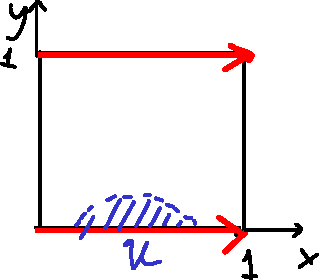
\includegraphics[width=\linewidth]{hom_surface_square.pdf}
\end{minipage}
\begin{minipage}{0.6\textwidth}
    Склеим горизонтальные стороны квадрата как нарисовано.
    $(x,0) \sim (x,1)$, а остальные эквиваленты только себе.
\end{minipage}

\begin{center}
    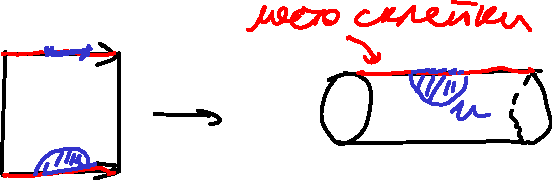
\includegraphics[width=0.7\linewidth]{hom_surface_cylinder.pdf}
\end{center}
$U$ открыто в квадрате, $U$ не открыто в цилиндре, т.к. $p^{-1}(U)$ не открыто.

Лента Мёбиуса:
\begin{center}
    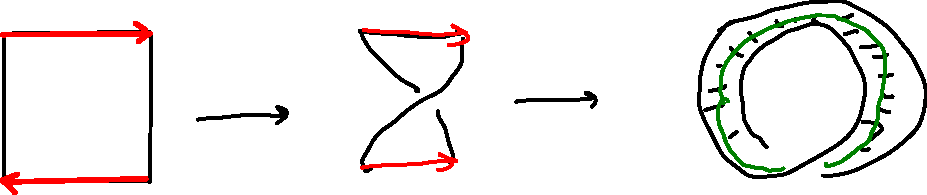
\includegraphics[width=0.7\linewidth]{hom_surface_mobius.pdf}
\end{center}
Свойства ленты Мёбиуса:
\begin{itemize}
    \item только одна сторона
    \item только один край
    \item средняя линия не делит на части
    \item на ленте Мёбиуса можно нарисовать полный граф на шести вершинах без пересечения ребер (упражнение) [На плоскости только $K_4$]
    \item на ленте Мёбиуса любая карта красится в 6 цветов (довольно просто) [Для плоскости 4 цвета, очень сложно]
\end{itemize}

\begin{theorem}[Жордана]
    Замкнутая непересекающаяся кривая на плоскости делит плоскость ровно на две компоненты связанности.
    Ровно одна из них ограниченна.
\end{theorem}

\begin{theorem}[Эйлера]
    Для плоскости:
    \begin{multline*}
        (\text{количество вершин}) + (\text{количество граней}) =\\
        = (\text{количество ребер}) + 2
    \end{multline*}
    (для связного графа с непересекающимися ребрами)

    Для ленты Мёбиуса:
    \[\text{В} + \text{Г} = \text{Р} + \chi\]
    где $\chi = 1$, если есть цикл, опоясывающий ленту, или $2$.
\end{theorem}

Тор:
\begin{center}
    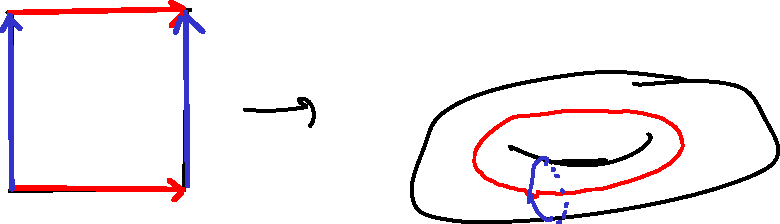
\includegraphics[width=0.7\linewidth]{hom_surface_torus.pdf}
\end{center}

Бутылка Клейна:
\begin{center}
    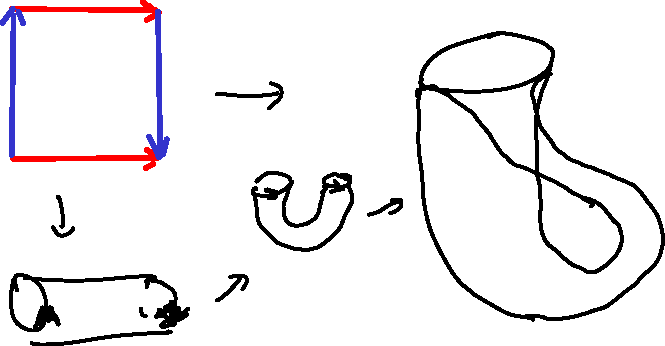
\includegraphics[width=0.7\linewidth]{hom_surface_klein_bottle.pdf}
\end{center}
Бутылка Клейна -- это 2 склеенные ленты Мёбиуса:
\begin{center}
    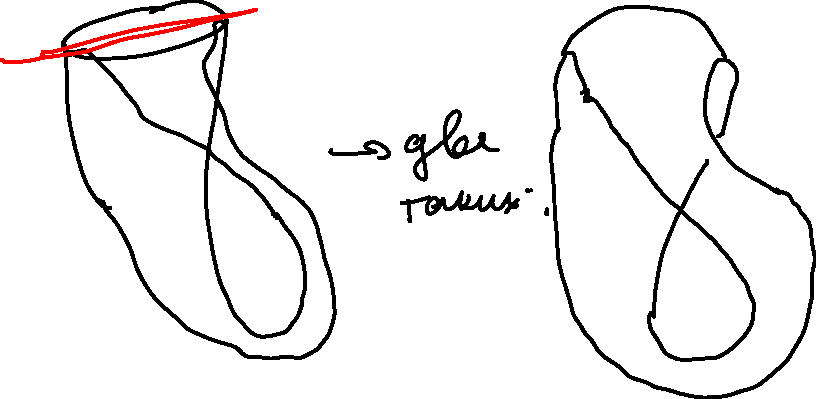
\includegraphics[width=0.7\linewidth]{hom_surface_klein_bottle_glue.pdf}
\end{center}

\begin{enumerate}
    \item Проективная плоскость
          \begin{center}
              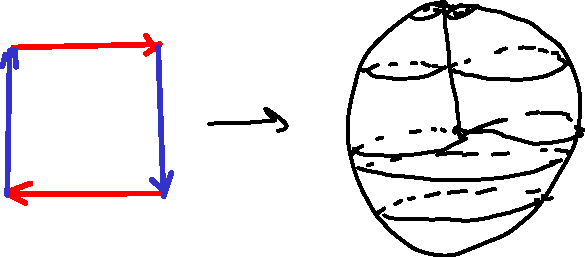
\includegraphics[width=0.7\linewidth]{hom_surface_klein_rp1.pdf}
          \end{center}
          Другие интерпретации проективной плоскости ($\R P^2$):
    \item $x \sim -x$ ($x$ -- крайняя точка круга)
          \begin{center}
              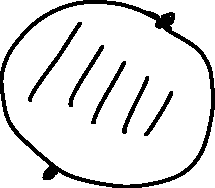
\includegraphics[width=0.3\linewidth]{hom_surface_klein_rp2.pdf}
          \end{center}
    \item $S^2/ x\sim -x$
          \begin{center}
              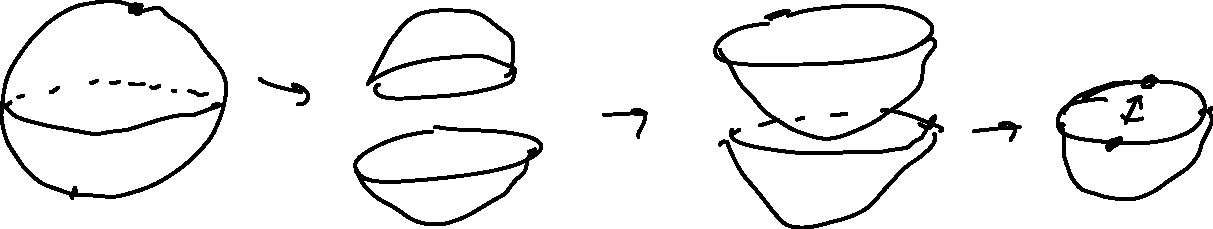
\includegraphics[width=0.9\linewidth]{hom_surface_klein_rp3.pdf}
          \end{center}
    \item $\R^3 \setminus \{(0,0,0)\} / (x,y,z) \sim (\lambda x; \lambda y; \lambda z)$
    \item Множество прямых в $\R^3$, проходящих через $(0,0,0)$. Метрика - угол между прямыми
    \item $\{[x:y:z] : x,y,z \in \R,\ x^2 + y^2 + z^2 \neq 0\}$ -- однородные координаты: $[x:y:z] = [\lambda x: \lambda y: \lambda z]$.
          $Ax + By + Cz = 0$ -- уравнение любой прямой на проективной плоскости
    \item $\R P^2 = \R^2 \cup \R^1 \cup \R^0$
          \begin{center}
              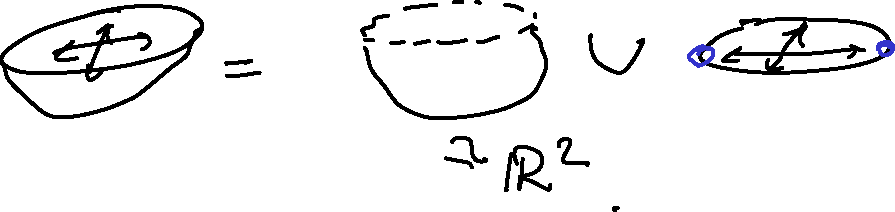
\includegraphics[width=0.7\linewidth]{hom_surface_klein_rp7.pdf}
          \end{center}
\end{enumerate}

Сфера:
\begin{center}
    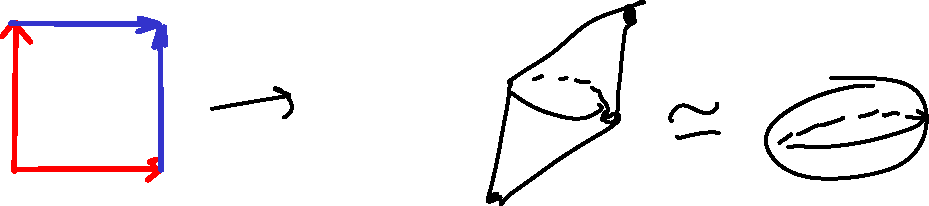
\includegraphics[width=0.7\linewidth]{hom_surface_sphere.pdf}
\end{center}
Упражнение: что будет, если склеить по-другому?
\begin{center}
    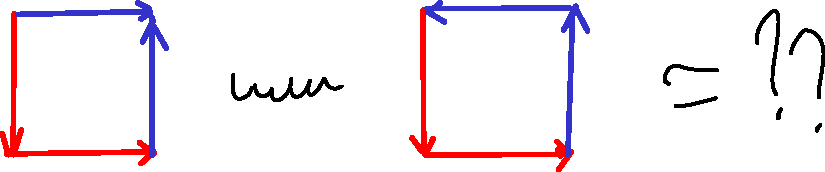
\includegraphics[width=0.7\linewidth]{hom_surface_unknown.pdf}
\end{center}
Еще: Если ленту повернуть на 2 полуоборота и склеить, то получится лента, гомеоморфная обычной.
(в $\R^2$ не очевидно, в $\R^4$ переводится -- упражнение)
\begin{center}
    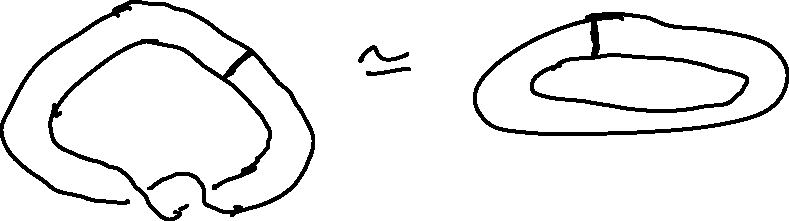
\includegraphics[width=0.7\linewidth]{hom_surface_mobius_hom.pdf}
\end{center}

Поверхности:

Поверхность можно задать, если есть многоугольник.
Приклеивание ручки (тора):
\begin{center}
    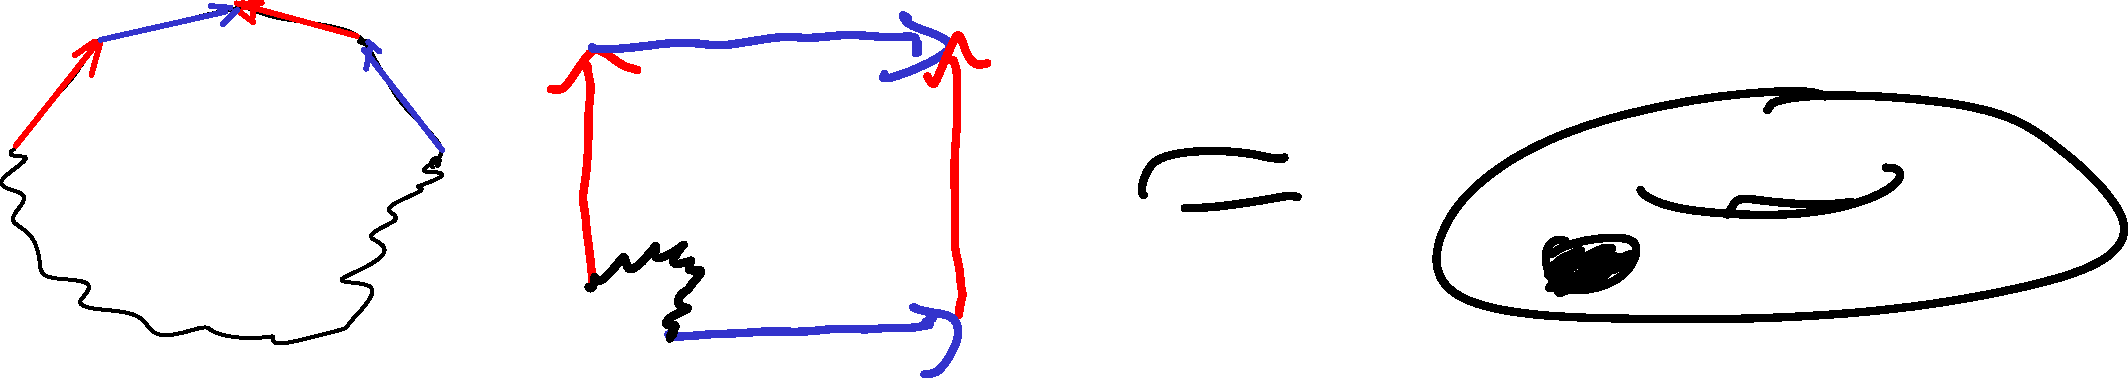
\includegraphics[width=0.7\linewidth]{hom_surface_glue_handle.pdf}
\end{center}
Приклеивание пленки (ленты Мёбиуса):
\begin{center}
    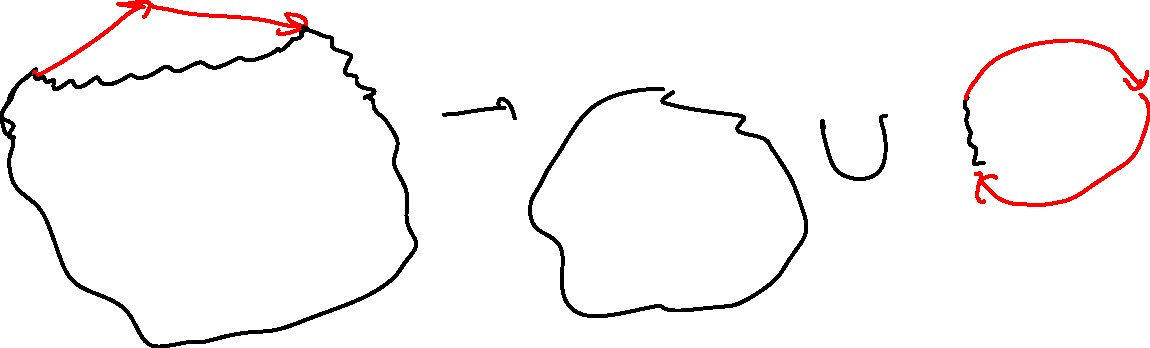
\includegraphics[width=0.7\linewidth]{hom_surface_glue_wrap.pdf}
\end{center}

Почему проективная плоскость с дыркой это лента Мёбиуса?
Край ленты Мёбиуса -- окружность.
\begin{center}
    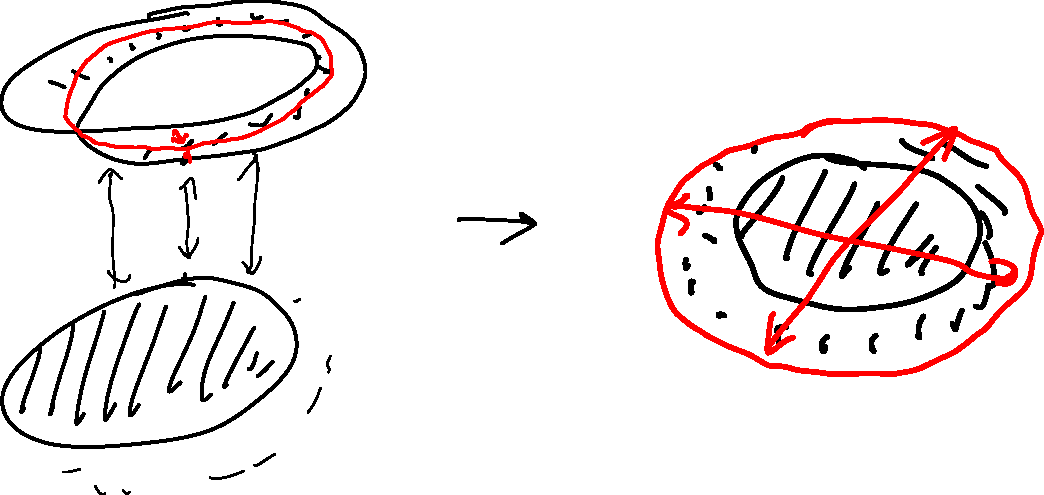
\includegraphics[width=0.7\linewidth]{hom_surface_circle_mobius.pdf}
\end{center}

\begin{theorem}
    (почти) Любая двумерная поверхность -- либо сфера с $k$ ручками, либо проективная плоскость с $k$ ручками, либо бутылка Клейна с $k$ ручками.
\end{theorem}

Проективная плоскость -- сфера с пленкой, бутылка Клейна -- сфера с 2 пленками.

\begin{example}
    Приклеивание. $X, Y$ -- топологические пространства.
    $A \subset X, f: A \to Y$ -- непрерывное отображение.

    Приклеивание: $X \sqcup_f Y = X \sqcup Y / a \sim f(a)$.
    \begin{center}
        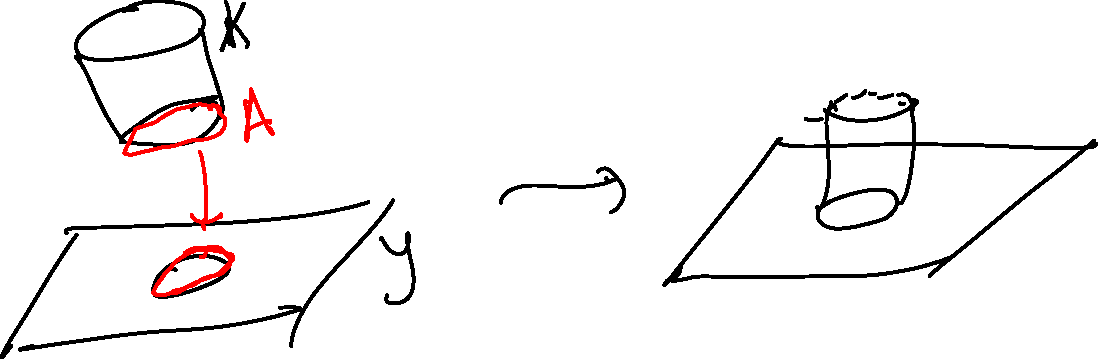
\includegraphics[width=0.7\linewidth]{hom_surface_gluing.pdf}
    \end{center}
\end{example}
\end{document}